\chapter{Signal to noise ratio of filtered photodetection signals}
\label{ch:snr}

The DarkSide20k detectors will use photodetector modules (PDMs) made up from
many silicon photomultipliers (SiPMs). For what concerns us, the output is
similar to a single SiPM output. When a photon hits the photomultiplier, the
electrical output is a sudden current spike, with a rise time on the order of
nanoseconds, which decays slowly in some microseconds.

Each SiPM is made up of many single photodiodes (called ``cells''), so when
different photons hit simultaneously different cells, the output is a signal
with an amplitude proportional to the number of photons. See
\autoref{fig:signals} for an example.

\marginpar{Bibliography for the SiPM.}

\begin{figure}
    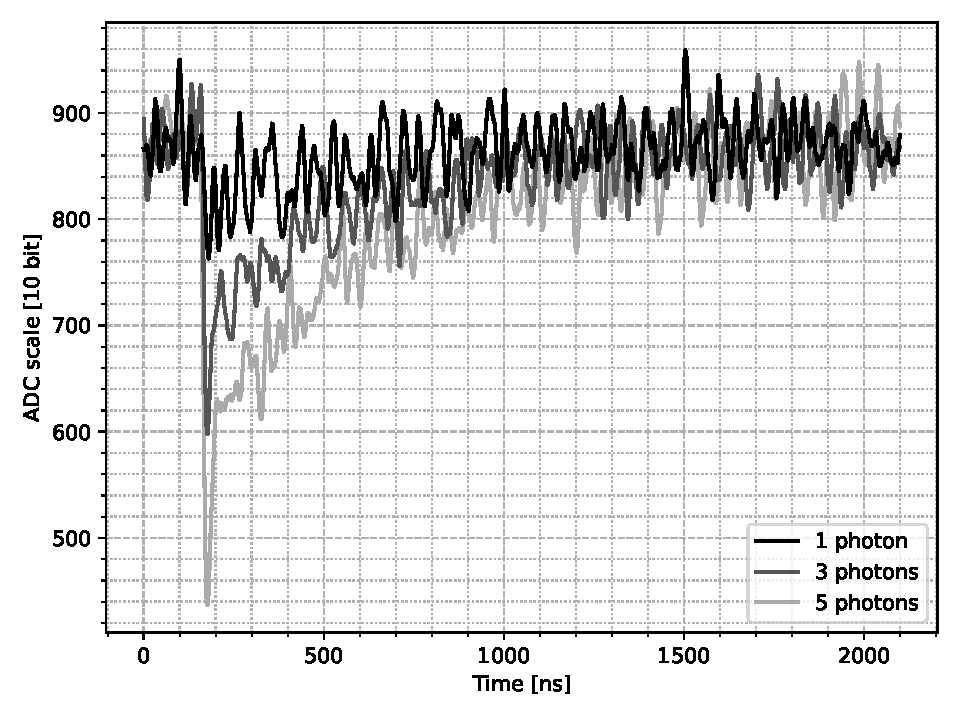
\includegraphics[width=\textwidth]{figsignals}

    \figcaption{signals}{Example PDM signals taken from the LNGS test data
    (\autoref{sec:lngsdata}). The different curves correspond to an increasing
    number of photons being detected simultaneously, with the resulting signal
    being the sum of single-photon signals. Notice that the noise amplitude is
    the same in all curves, which means that it is produced mostly outside of
    the PDM.}

\end{figure}

Our goal is to study the performance of some filters in finding and measuring
the amplitude of the signals amidst electrical noise. We'll now introduce the
dataset, list the filters tested, define a performance measure and show the
results. Finally we'll compute and comment the noise spectrum. The code for
this work is online at \url{https://bitbucket.org/Gattocrucco/sipmfilter}.

\section{Data}
\label{sec:lngsdata}

For this study we used test data taken at liquid nitrogen temperature from a
setup in the Gran Sasso National Laboratories (LNGS). A laser pulse is shot at
regular time intervals on the PDM. Both the laser trigger and the detector
output are sampled at \SI{1}{GSa/s} with a 10 bit ADC and saved separating the
data in ``events'' where each event correspond to a single laser pulse. See
\autoref{fig:lngs}.

\marginpar{Bibliography for the LNGS data. Maybe add a 2D histogram of the
data.}

\begin{figure}
    \hspace{-0.26\textwidth}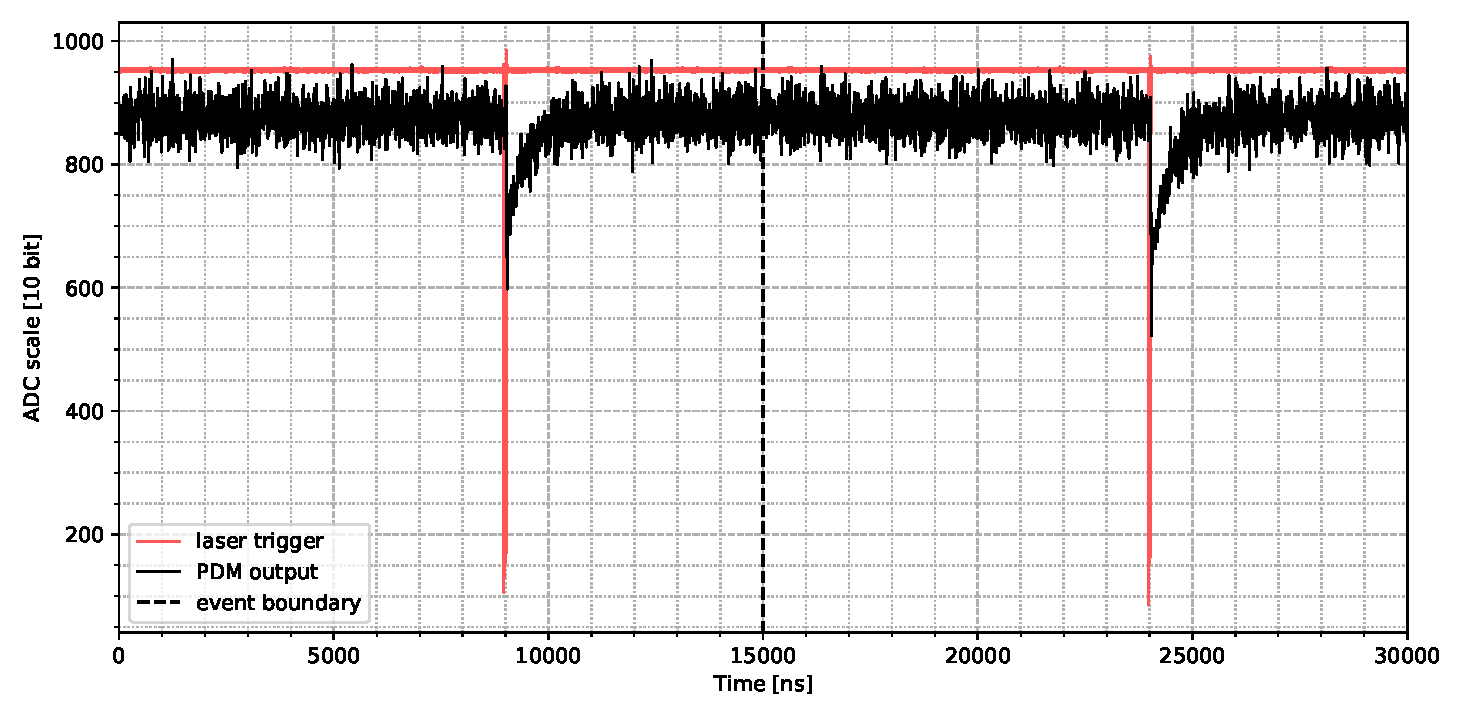
\includegraphics[width=1.52\textwidth]{figlngs}
    
    \figcaption{lngs}{A pair of events from the LNGS test data
    (\autoref{sec:lngsdata}).}

\end{figure}

We used the PDM slot 8 data, which as per \autoref{fig:pdmadcch} corresponds
to Tile 57 which means the data is in the directory
\url{http://ds50tb.lngs.infn.it:2180/SiPM/Tiles/FBK/NUV/MB2-LF-3x/NUV-LF_3x_57/}. We used the file \nolinkurl{nuvhd_lf_3x_tile57_77K_64V_6VoV_1.wav}.

\marginpar{Slot 8 probably is just a Proto0 name, should mention it later. And
what are these ``tiles''?}


In the dataset there are a couple of problems. The first is that signals with
many photoelectrons saturate, however this won't trouble us since we'll need
only single photoelectron signals. The second is the presence of some spurious
signals which do not correspond to the laser pulse. I filtered these out by
putting a threshold in the part of each event \emph{before} the laser trigger,
which should be flat apart from the noise; there were 72 of them out of
\num{10005} events.

In principle a spurious signal arriving \emph{after} the ``official''
laser-induced signal matters too, however I'm ignoring them out of this logic:
spurious signals hitting earlier raise the official signal in a somewhat
uniform way with their slowly decaying tail, so the detected amplitude will
have a bias which is significant, but possibly small and as such not
identifiable. Spurious signals hitting later will add a large spike in the tail
of the official signal, so the amplitude will be noticeably higher, such that a
single photoelectron pulse gets confused as a double or higher one, and
we'll automatically ignore it as we'll consider signals detected as single.

This reasoning may fail depending on the details of filtering and the specific
relative timing of the signals, however the final most important consideration
is that I expect less than 100 spurious late pulses since there are 72 early
ones and the laser pulse is in the middle of the event, so less than \SI1\%.
See \autoref{fig:spurious} for some examples of spurious/saturated signals.

\marginpar{The afterpulse stuff I had not understood properly may change all
this.}

\begin{figure}
    \hspace{-0.26\textwidth}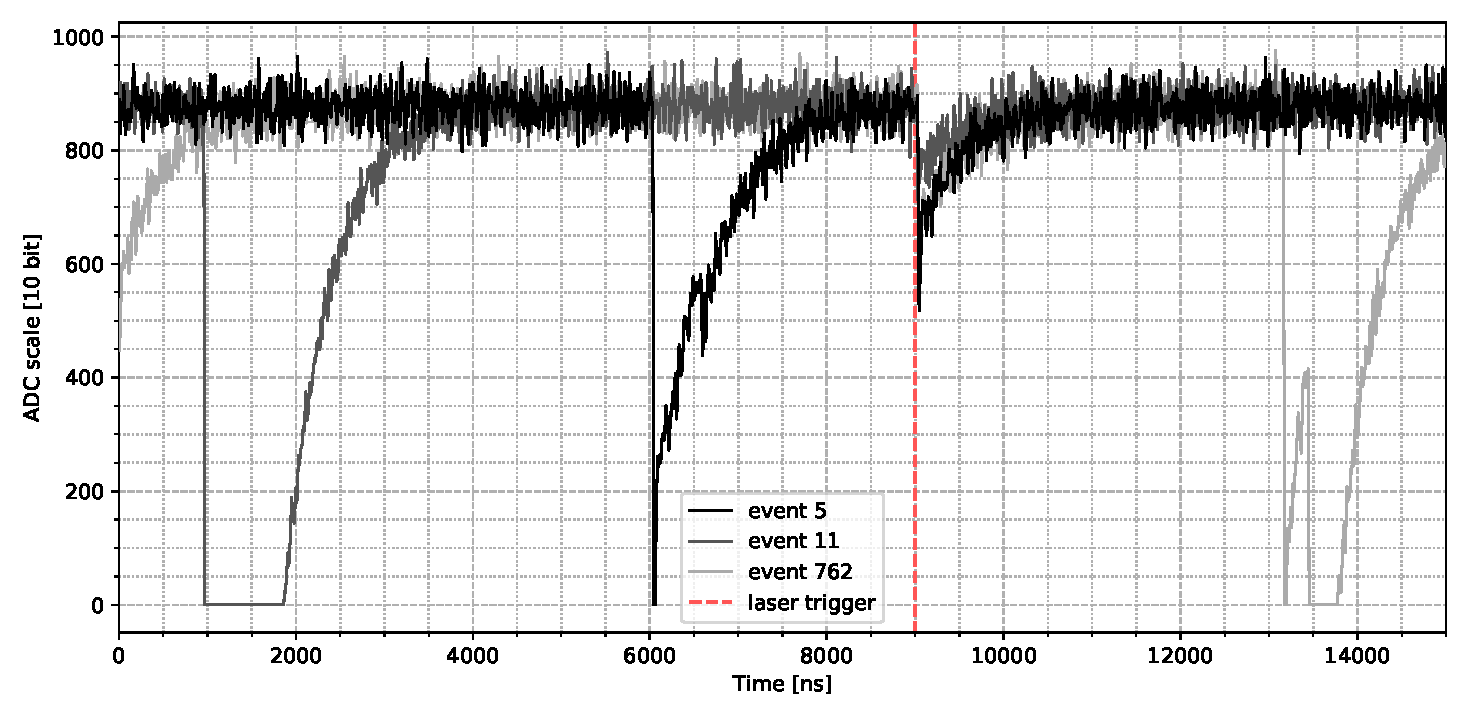
\includegraphics[width=1.53\textwidth]{figspurious}
    
    \figcaption{spurious}{Examples of spurious signals in the LNGS test data
    (\autoref{sec:lngsdata}).}

\end{figure}

\section{Filters}
\label{sec:filters}

A filter operates by converting the original sequence of ADC samples $(x_1,
x_2, \ldots)$ to a new ``filtered'' sequence $(y_1, y_2, \ldots)$. The filters
are causal, i.e. the filtered sample $y_n$ can be computed only using the
original samples up to $x_n$. This limitation is because we are interested in
using the filters online, i.e.\ produce the filter output continuously as
samples are read.

We tested three filters: the moving average, the exponential moving average or
autoregressive filter, and the cross-correlation filter.

The moving average consists in taking the average of the last $N$ samples:
%
\begin{equation}
    y_n =  \frac1N \sum_{i=1}^N x_{n-N+i}.
\end{equation}

The exponential moving average weighs past samples with an exponentially
decaying coefficient, and can be written recursively as
%
\begin{equation}
    y_n = a y_{n-1} + (1 - a) x_n, \quad a \in (0, 1).
\end{equation}
%
The scale of the exponential decay is given by
%
\begin{align}
    \tau &= -\frac1{\log a}, \\
    &\approx \frac1{1-a} \text{ for $a$ close to 1.}
\end{align}

The cross-correlation filter is the most sophisticated we considered. Let
$\mathbf h = (h_1, h_2, \ldots, h_N)$ be a \emph{template} of the signal
waveform we want to detect. This means $\mathbf h$ should ideally match the
shape of the signal waveform we want to find in the noisy data. The filter is
then the cross-correlation of $\mathbf x$ with $\mathbf h$:
%
\begin{equation}
    y_n = \sum_{i=1}^N h_i x_{n-N+i}.
\end{equation}
%
Under the assumption that the data is white noise plus a signal that perfectly
matches the template apart from amplitude, this filter is optimal in the sense
that in the filter output there will be a peak corresponding to the signal and
this peak will have the maximum possible height relative to the standard
deviation of the filtered noise.

The differences we have from the ideal case are:
%
\begin{enumerate}
    \item the shape of the signal probably changes a bit each time;
    \item the signal is not aligned always in the same way to the ADC timebase;
    \item the noise is not white.
\end{enumerate}

The variation of the actual signal shape is difficult to address directly. The
noise spectrum can be corrected by appropriately transforming $\mathbf h$, in
this case the filter is called \emph{matched filter}. Let $\mathbf s$ and
$\mathbf w$ be the signal and noise, such that the waveform to be filtered is
$\mathbf x = \mathbf s + \mathbf w$. Let $R$ be the noise covariance matrix,
i.e. $R_{ij} = \operatorname{Cov}[w_i, w_j]$. Then the template for the matched
filter is
%
\begin{equation}
    \mathbf h_\text m = R^{-1} \mathbf h.
    \label{eq:matched}    
\end{equation}

\marginpar{Explain that the matched filter is equivalent to rank~1 least
squares. As a general ref for the matched filter, use fer15.}

We tried implementing the matched filter with mixed results we will not report
in detail. We computed the noise covariance matrix on the event samples before
the signal. Since the noise is stationary, $R$ is a Toeplitz matrix, i.e. the
covariance depends only on the lag between two samples.
\autoref{fig:autocorrlngs} shows the noise covariance obtained.

\marginpar{Add the autocorrelation of the Proto0 noise to the plot.}

\begin{figure}
    \widecenter{\includempl{figautocorrlngs}}
    
    \figcaption{autocorrlngs}{Autocorrelation of the LNGS test data noise,
    computed on the part of the events before the trigger. The autocorrelation
    at lag $t$ is the correlation between a sample and another sample occurring
    a time $t$ after the first. The standard deviation of the noise is 26.7 ADC
    units.}

\end{figure}

The matched filter worked slightly better than the cross-correlation filter, as
expected, but only for $N$ sufficiently small, getting worse as $N$ increased.
This could be due to numerical accuracy problems in solving the linear system
$R$ in \autoref{eq:matched}, or in computing $R$. We didn't work on this
further since the gain is probably small.

\marginpar{Expand on the numerical issues. The uncorrected template is local,
while the template corrected for noise is less local and has large
cancellations.}

We computed the template for the cross-correlation filter by taking the median
of single photoelectron signals. We did not align the signals, we operated as
if they occurred always with the same alignment relative to the event time
window. The template obtained is shown in \autoref{fig:template}. When using
the template, we normalize it to unit sum such that the output from the
cross-correlation filter is comparable to the output from the moving averages,
i.e. if we send a flat waveform into the filter, the output has the same value
as the input.

\marginpar{Use the template from the second chapter; plot the template without
alignment, with trigger, with filtering; explain that we use 1 pe pulses to
avoid afterpulses; cite Luzzi to say it should not matter much how we compute
the template in detail.}

\marginpar{Explain that we fix the mean-like behaviour for all filters because
we have to subtract the baseline.}

Since we will try various lengths of the filter template, we have to decide how
to truncate the full template. When truncating to $N$ samples, we pick $N$
contiguous samples from the template such that their sum is the minimum
possible (recall the template is negative). Of course normalizing the template
to unit sum is done after truncation.

\begin{figure}
    \widecenter{\includempl{figtemplate}}
    
    \figcaption{template}{The template used for the cross-correlation filter.
    It is the median of unaligned single photon events from the LNGS test data.}

\end{figure}

See \autoref{fig:filters} for an example of filter output.

\begin{figure}
    \widecenter{\includempl{figfilters}}
    
    \figcaption{filters}{An event from the LNGS test data filtered with the
    three filters used. The number of averaged samples in the moving average
    filter, the scale of the autoregressive filter, and the length of the
    template of the cross-correlation filter are all 1024 samples (at
    \SI1{GSa/s}).}

\end{figure}

\section{The fingerplot}
\label{sec:fingerplot}

To measure the performance of filters, we define a signal to noise ratio (SNR)
as follows: the SNR is the ratio of the average peak filter output value for
single photon signals over the standard deviation of the filtered noise.

We could consider other similar measures, for example we could include the
standard deviation of the peak filter output value since that influences where
we should place a threshold to discriminate signals, however it is sufficient
to use any reasonable definition for the purpose of comparing different
filters. Effectively we computed the SNR without exactly respecting the
definition above, we'll see in detail.

For each event we compute the filter output at a fixed temporal delay from the
leading edge of the laser trigger pulse (see \autoref{fig:filtersample}).
Then we compute the average of the samples before the trigger pulse and take
that value as ``baseline''. We subtract the baseline from the filter output,
and finally we change the sign to obtain positive values since the signals are
negative.

\begin{figure}
    \widecenter{\includempl{figfiltersample}}
    
    \figcaption{filtersample}{Example of how a signal amplitude is computed in
    an event for the purpose of computing the SNR. The samples in the shaded
    region are averaged to compute the baseline. The filter is evaluated at a
    fixed offset (indicated by the arrow) from the leading trigger edge. The
    amplitude then is the difference between the baseline and the filter value.
    The shaded region ends 100 samples before the trigger.}

\end{figure}

We take the list of these baseline and sign corrected filter outputs and
compute an histogram. One of these histograms is shown in
\autoref{fig:fingerplot}. It is called ``fingerplot'' due to the descending
peaks reminding of fingers.

\begin{figure}
    \widecenter{\includempl{figfingerplot}}
    
    \figcaption{fingerplot}{The fingerplot for the moving average filter with
    128 samples evaluated 128 samples after the trigger.}

\end{figure}

The first peak is centered on zero and thus corresponds to cases where the
laser pulse produces no photoelectrons. Since the instant where we are
evaluating the filter output in each event is independent of the output itself
(instead of e.g.\ being determined by peak finding), this peak is the
distribution of the noise after passing through the filter.

The various other peaks correspond to an increasing number of photons. The
second peak is the distribution of the filter output at a fixed instant for
single photon signals. Assuming for the moment that the instant where we
evaluate the filter yields the highest signal response, this means that the SNR
is the mean of the second peak divided by the standard deviation of the first.

Since the peaks are often overlapping, and that we will have to repeat the
calculations for many fingerplots automatically without checking each one, we
use robust measures of location and scale instead of the average and standard
deviation. We run a peak finding algorithm on the histogram and divide the data
by putting boundaries midway between peaks, so that we assign each datapoint to
a peak. For the second peak, we take the median instead of the average. For the
first peak, we take the half symmetrized \SI{68}\% interquantile range instead
of the standard deviation, i.e.\ half the difference between the 0.84 and 0.16
quantiles. On a gaussian distribution these are equivalent to the mean and
standard deviation, however they are less sensible to messing up the tails of
the distribution, which happens since the boundaries cuts away the tails and
there is contamination from the tails of the neighbouring peaks.

\marginpar{Mention that I'm always checking that the median of the 0 pe peak
is zero within its error.}

\section{SNR versus filter length}

When determining how to compute the SNR from the fingerplot we assumed that we
were evaluating the filter output at the optimal instant. Since we do not know
it a priori, we repeat the computation for a range of values of the filter
evaluation point. A simpler solution that comes to mind is taking the minimum
(the signals are negative) of the filter output in each event, however this
would bias upward the SNR measure because the minimum can yield lower values
due to noise peaks. Instead, by fixing the point independently from the data,
the random oscillation due to noise is symmetrical and the averaging recovers
the actual amplitude of the filter output for the signal.

The resulting SNR curves are shown in \autoref{fig:snrplot}, repeated for a
range of values of the filters length parameter. For the moving average and
cross-correlation filter, the length parameter is the number of samples, $N$.
For the exponential moving average, it is the scale of the exponential decay
$\tau$.

\begin{figure}
    \widecenter{\includempl{figsnrplot}}
    
    \figcaption{snrplot}{The SNR as a function of delay from trigger (x-axis)
    and filter length (shade of gray) for the three filters.}

\end{figure}

The maximum of each curve gives the actual SNR figure we are interested in. We
expect by intuition that the width of the maximum is approximately proportional
to the temporal resolution we could achieve if we used the filter output to
locate temporally the signal. So we do another plot
(\autoref{fig:snrmaxplot}) where we show the maximum SNR value and the width
of the peak versus the filter length parameter. We measure the width as the
distance between the two points where the SNR is 1 less than its maximum value.

\marginpar{I can drop the snrmaxplot because it's already in the baseline
effect plot.}

\begin{figure}
    \widecenter{\includempl{figsnrmaxplot}}
    
    \figcaption{snrmaxplot}{Top plot: maximum SNR achieved with each filter
    (different curves) and filter length (x-axis). Bottom plot: the width of
    the maxima, computed as the length of the interval of offset from trigger
    with endpoints where the SNR is 1 less than the maximum. The
    cross-correlation filter mantains almost constant width with increasing
    SNR, while the other two filters have increasing width.}

\end{figure}

\section{Effect of the baseline computation}

In constructing the fingerplot, we subtract from the filter output value the
baseline, i.e.\ the average value of the waveform in absence of signals. We
compute the baseline for each event as the average of the samples before the
signal. More precisely, we averaged \num{8000} samples. The value obtained
varies randomly due to the noise; its standard deviation is that of the noise
divided by $\sqrt{8000}$. The maximum filter length we use is 2000, so in that
case the width of the peaks gets an additional contribution (summed in
quadrature) which is $\sqrt{2000/8000} = 1/2$ of the width we would have with a
noiseless baseline, i.e.\ the width of the first peak is $\sqrt{1 + 1/2} - 1 =
\SI{22}\%$ larger, lowering the SNR by the same percentual.

This is not just a problem of this test that can be worked around in the real
application, because how the baseline is computed is a relevant part of the
signal finding, since it requires either a fast on-digitizer algorithm
estimating it reliably or sending enough samples to subsequent stages in the
data processing chain.

To get an idea of the effect of the baseline, we repeat everything computing
the baseline with just 1000 or 200 samples. The result is in
\autoref{fig:changebs}. We see that, for example, going from 8000 to 200
baseline samples the maximum SNR drops from about 20 to about 9.

\marginpar{The effect of a shorter baseline should be described analytically
with a sum in quadrature, check and explain this.}

\marginpar{Explain why the SNR of the cross correlation filter drops with
increasing filter length when the baseline is short. The filter behaves like
a mean, so its peak value drops as it gets longer; the noise rms decreases too
but gets a constant contribution from the baseline variance.}

\begin{figure}
    \widecenter{\includempl{figchangebs}}
    
    \figcaption{changebs}{The same plot of \autoref{fig:snrmaxplot} repeated
    changing the number of pre-signal samples used to compute the baseline. The
    left column is the same data from \autoref{fig:snrmaxplot}, with 8000
    baseline samples. The performance decreases with a lower number of samples
    because the standard deviation of the baseline increases and the baseline
    is compared to the filtered signal amplitude to discriminate signals.}

\end{figure}

\section{Noise spectrum}
\label{sec:spectrum}

We take the region of each event before the trigger pulse, compute its
periodogram, and take the median across events for each frequency. We use the
median instead of the average in case there were spurious signals or
irregularities we missed. We do the same for data obtained with the same sensor
but when it was in the Proto0 setup, biased below breakdown voltage and sampled
at \SI{125}{MSa/s}. We thus obtain two plausible noise spectra, shown in
\autoref{fig:spectra}.

\marginpar{In the caption of \autoref{fig:spectra} I say that the Proto0 data
is at room temperature, but probably it's liquid Argon.}

\marginpar{Source and details of the Proto0 noise data.}

\begin{figure}
    
    \widecenter{\includempl{figspectra}}
    
    \figcaption{spectra}{Spectrum for the PDM we used in the LNGS test data,
    both in the LNGS test data setup and in the Proto0 detector setup. While
    the LNGS data is in working conditions at liquid nitrogen temperature, the
    Proto0 data we used was taken at room temperature with sensors biased below
    breakdown voltage for the purpose of measuring noise.}

\end{figure}

We said the cross-correlation filter is optimal if the noise is white.
Actually, it is sufficient that the noise spectrum is flat in the support of
the signal spectrum, because if we filtered away frequencies outside of it, all
the signal would still be in the waveform. In \autoref{fig:templsp} we show
the power spectrum of the signal and its integral. We see that \SI{90}\% of it
is below XXX~\si{MHz}, which corresponds to an approximately flat region in the
noise spectra. This means that the cross-correlation filter is close to
optimal.

\marginpar{False: most of the signal spectrum is in the rapidly ascending part
of the noise spectra.}

\marginpar{I should explain why you must not use windowing for the Fourier
transform of the pulse. It is not stationary.}

\begin{figure}
    
    \widecenter{\includempl{figtemplsp}}
    
    \figcaption{templsp}{Comparison of the spectra of signal and noise. The red
    curve shows the percentual of signal power below a given frequency. The
    signal spectrum is computed with the discrete Fourier transform of the
    cross-correlation filter template (\autoref{fig:template}) without
    windowing.}

\end{figure}
